\documentclass[12pt]{report}
\usepackage[french]{babel}
\usepackage[utf8]{inputenc}
\usepackage[T1]{fontenc}
\usepackage[top=2cm, bottom=2cm, left=2cm, right=2cm]{geometry}
\usepackage{graphicx}
\usepackage{xcolor}
\usepackage{float}
\usepackage[french, onelanguage, boxruled, longend]{algorithm2e}
\usepackage{setspace}
\usepackage{multirow}
%\usepackage{algorithm}
%\usepackage{algorithmic}

\newcommand{\HRule}{\rule{\linewidth}{0.5mm}}

\begin{document}
    \begin{titlepage}
        \begin{center}
            \textbf{République Algérienne Démocratique et Populaire}\\
            \textbf{Ministère de l'Enseignement Supérieur et de la Recherche Scientifique}\\[1cm]
            
            
\includegraphics[scale=0.5]{./ressources/USTHB_Logo.png}\\[1cm]
            
            \large
            \textbf{Université des Sciences et de la Technologie Houari Boumédiène}\\[0.5cm]
            \textbf{Faculté d'Electronique et d'Informatique}\\
            \textbf{Département Informatique}\\[0.5cm]

            \Large
            \textbf{Master Systèmes Informatiques intelligents}\\[0.5cm]
            
            \textbf{Module :} Conception et Complexité des Algorithmes

            \HRule \\[0.4cm]
            \LARGE{\textbf{Rapport de projet de TP}\\
            \textit{}\\[0.4cm]}
            \HRule \\[2cm]
            
            \large
            \textbf{Réalisé par :}\\
            AIT AMARA Mohamed, 181831072170\\
            BOUROUINA Rania, 181831052716\\
            CHIBANE Ilies, 181831072041\\
            HAMMAL Ayoub, 181831048403
            
            \vfill
            Année universitaire : 2021 / 2022
        \end{center}
    \end{titlepage}
    \normalsize

    \newpage
    \onehalfspacing
    \chapter{Recherche séquentielle d'un élément dans un tableau}

\section{Description de l'objectif de l'algorithme}
En informatique, un tableau est une structure de données représentant une séquence finie d'éléments défini par un index représentant sa position au sein du tableau nous permettant d'y accéder. C'est un type de conteneur que l'on retrouve dans un grand nombre de langages de programmation et est l'un des plus utilisés du de sa simplicité.
\par
Les données du tableau étant accessible individuellement il est nécessaire de faire une recherche lorsque l'on souhaite accéder a une valeur spécifique du tableau cependant lorsque la taille de la structure est grande il devient difficile d'y accéder efficacement. Dans ce chapitre on nous allons voir la recherche séquentielle qui est une recherche très coûteuse en temps et nous allons aussi présenter une optimisation de cette recherche afin de gagner en complexité temporelle.
\par
La recherche séquentielle ou recherche linéaire est un algorithme pour trouver une valeur dans une liste ou un tableau. Elle consiste simplement à considérer les éléments du tableau les uns après les autres, jusqu'à ce que l'élément soit trouvé, ou que toutes les cases aient été lues. Elle est aussi appelée recherche par balayage.. (voir Figure \ref{fig:recherche_sec}).

\begin{figure}[H]
    \centering
        \includegraphics[scale=0.5]{./ressources/Recherche_séquentielle.jpg}
        \caption{Exemple graphique d'une recherche séquentielle}
    \label{fig:recherche_sec}
\end{figure}

\section{Fonctionnement de l'algorithme}
La recherche séquentielle consiste à prendre les éléments du tableau les uns après les autres, jusqu'à avoir trouvé la cible, ou avoir épuisé le tableau.Elle ne demande aucune condition au préalable pour le tableau en entrée; par exemple: il n'est pas necessaire que le tableau soit trié.


\par
Nous pouvons le représenter via le pseudo code suivant :


\begin{function}[H]
    \textbf{Variables :}\\
    i : entier\;
    trouve : bool\;
    \Begin{
        $trouve \leftarrow faux $\;
        $i \leftarrow 0 $\;

         \While{$trouve \leftarrow false \:\: ET \:\: i \: < \: n$}
       {
            
            \If{$tab[i] == valeur$}{
                $trouve \leftarrow vrai $\;
                $i++$\;
            }
        }

            \uIf{$trouve \leftarrow vrai$}{
                $retourner\:\: i-1$\;
            }
            \Else {
             $retourner -1$\;
            }
}
    \caption{sequentielle(Entrée: tab: tableau d'entier; tailleTableau, valeur: entier;)}
\end{function}







\section{Calcul de complexité}
\subsection{Complexité temporelle}
La complexité de la recherche séquentielle est toujours égale à : $\mathcal{O}(n)$.

le tableau suivant représente les temps d'exécution théorique en nanoseconde de l'algorithme selon la variation de la taille de l'expression:

\small
\begin{center}
\begin{tabular}{| c | c | c | c | c | c | c | c | c | c | c | c | c |}
    \hline
    N & 10 & 50 & 100 & 500 & 1000 & 5000 & 10000 & 100000 & 1000000 & 10000000 \\
    \hline
    t(ns) & 10 & 50 & 100 & 500 & 1000 & 5000 & 10000 & 100000 & 1000000 & 10000000 \\
    \hline
\end{tabular}  
\end{center}

La figure suivante (voir Figure \ref{fig:temps_exec_th_algo2}) représente l'évolution du temps d'exécution théorique selon la longueur de l'expression.

\begin{figure}[H]
    \centering
        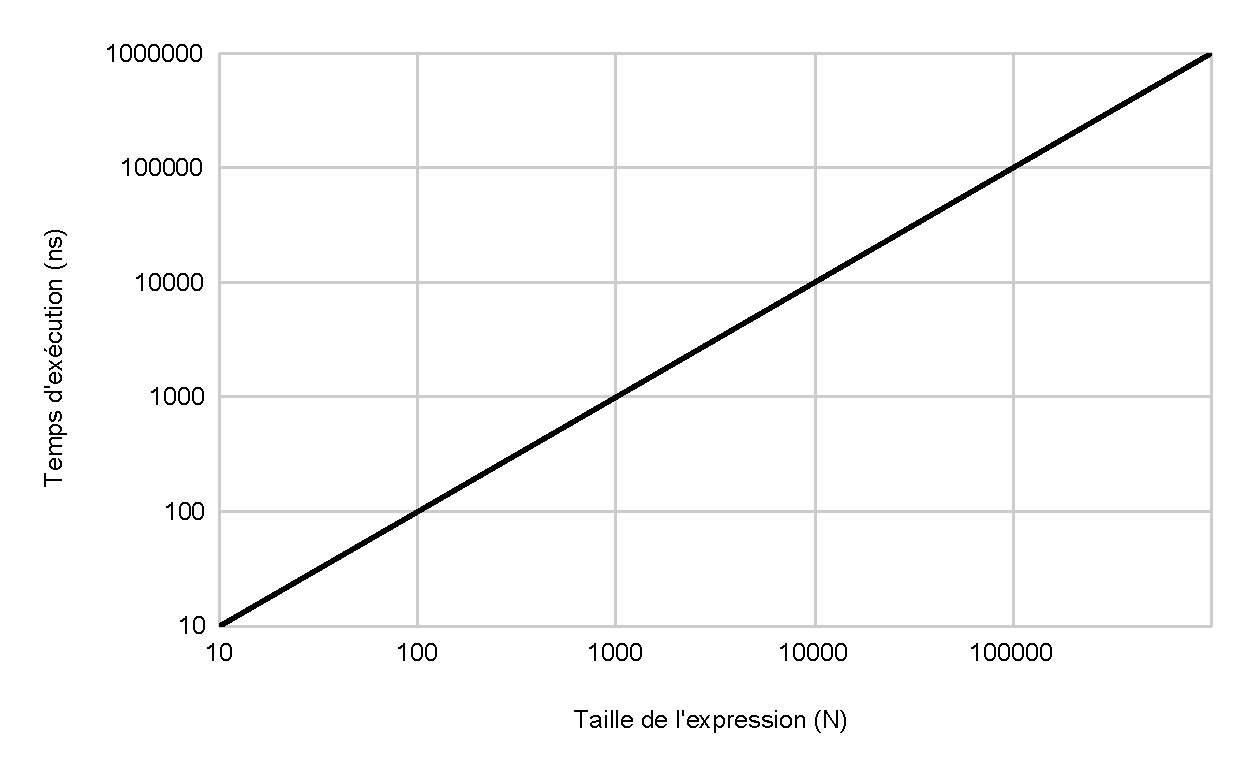
\includegraphics[scale=0.5]{./ressources/temps_execution_th_algo2.pdf}
        \caption{Temps d'exécution théorique de l'algorithme de recherche linéaire}
    \label{fig:temps_exec_th_algo2}
\end{figure} 

Depuis le graphe,  on observe que le temps d'exécution évolue de manière linéaire avec l'évolution de la taille de l'expression.


\subsection{Complexité spatiale}
\par
L'unique structure de données utilisée est un tableau d'entier a n éléments. 
\par
La taille d'un entier étant de 2 octets, la complexité spatiale est donc égale au produit de la taille du tableau et de la taille d'un entier : $n * 2 \approx \mathcal{O}(n)$
\par

\section{Expérimentation}
Le tableau suivant représente les temps d'exécution en nanoseconde de l'algorithme selon la variation de la taille de l'expression arithmétique en d'opérande.\\ \\
\small
\resizebox{19cm}{!}{
\begin{tabular}{| c | c | c | c | c | c | c | c | c | c | c | c | c |}
    \hline
    N &  10 & 50 & 100 & 500 & 1000 & 5000 & 10000 & 100000 & 1000000 & 10000000 \\
    \hline
    t1(ns) & 606 & 401 & 222 & 3224 & 12010 & 6864 & 106408 & 1066370 & 11130 & 11018 \\
    \hline
    t2(ns) & 866 & 1153 & 1851 & 5171 & 11383 & 52809 & 109357 & 1061730 & 3028000 & 38859000 \\
    \hline
    t3(ns) & 168 & 1066 & 1064 & 5714 & 10237 & 53084 & 2875 & 5070 & 4519680 & 56877700 \\
    \hline
    t4(ns) & 744 & 1119 & 1283 & 7111 & 747 & 2197 & 1504 & 11452 & 7636790 & 41331300 \\
    \hline
    t5(ns) & 588 & 785 & 829 & 1328 & 10459 & 3069 & 102717 & 1074940 & 1077270 & 54743600 \\
    \hline
    t6(ns) & 722 & 621 & 1402 & 1556 & 4204 & 10955 & 5509 & 1082590 & 1069420 & 11577 \\
    \hline
    t7(ns) & 638 & 499 & 375 & 5083 & 10259 & 6345 & 106589 & 493002 & 10463 & 38906200 \\
    \hline
    t8(ns) & 708 & 746 & 2192 & 7064 & 5008 & 8755 & 107439 & 1041410 & 1094640 & 40419900 \\
    \hline
    t9(ns) & 694 & 1225 & 1570 & 1118 & 11180  & 3275 & 122386 & 922361 & 10669 & 55940100 \\
    \hline
    t10(ns) & 666 & 1161 & 1504 & 2456 & 11349 & 10799 & 7470 & 1092110 & 7197500 & 40000300 \\
    \hline
    Moyenne(ns) & 2164 & 28704 & 92760 & 169733 & 341583 & 1047560 & 4598740 & 38774800 & 5626090000 & 37018600000 \\
    \hline
\end{tabular}}
\\
\normalsize
\par
La figure suivante (voir Figure \ref{fig:temps_exec_seq}) représente l'évolution du temps d'exécution selon la longueur du tableau.

\begin{figure}[H]
    \centering
        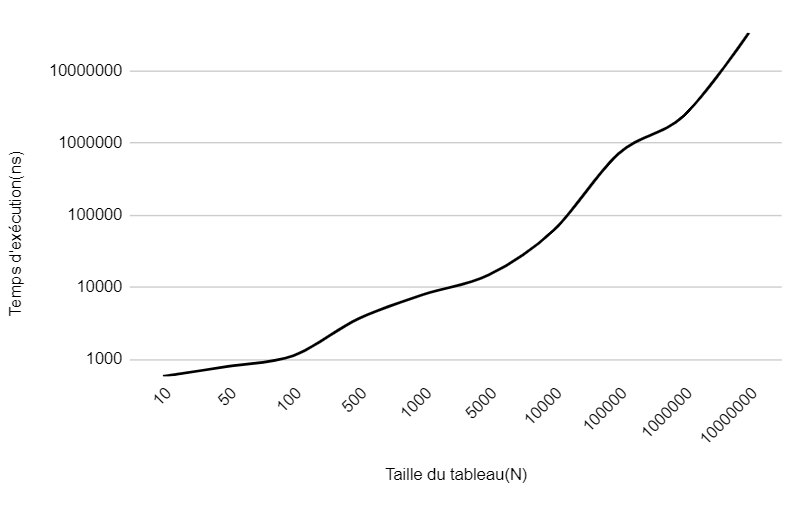
\includegraphics[scale=0.5]{./ressources/graphe_temps_execution.png}
        \caption{Temps d'exécution du programme selon la longueur du tableau}
    \label{fig:temps_exec_seq}
\end{figure}
\par
Depuis le graphe, la courbe est sous forme d'un arc ascendant, on observe que le temps d'exécution évolue de manière presque liénaire avec l'augmentation de la taille du problème, ce qui correspond bien à la complexité théorique calculée auparavant.
On a pas obtenu une droite linéaire car les testes étaient aléatoires.
\section{Amélioration}
L'algorithme de recherche linéaire est coûteux en terme de temps, donc on a pensé à utiliser 2 processus qui vont rechercher la valeur en parallèle pour gagner du temps.
Le premier processus commence à chercher depuis le début jusqu'à la moitié du tableau et le deuxième processus commence de la moitié jusqu'à la fin du tableau. Le premier d'entre eux qui trouve la valeur, il l'envoie au processus père.





\begin{function}[H]
    \textbf{Variables :}\\
    i, pos, status,debut,fin : entier\;
    $pid1, pid2, pid : pid_t$\;
    trouve : bool\;
    
    \Begin{
        $debut  \leftarrow 0$\;
        $fin  \leftarrow  tailleTableau/2 $\;
        $trouve  \leftarrow  faux $\; 
        
        $pid1 = fork()$\;\tcp{on crée le fils 1}
        \uIf {($pid1 == -1$)}{
        ecrire("y'a un problème lors de la création du fils 1")\;}
\Else{
\tcp{on commence la recheche du début jusqu'au milieu du tableau}
        \For{$i \leftarrow debut$ \KwTo $fin$}{
             \If{$tab[i] == valeur$}{
                $trouve \leftarrow vrai $\;
                $pos \leftarrow i$\;
            }
        }
\tcp{si le fils 1 trouve la valeur cherchée il affichera sa position sinon il affiche un nombre négatif}
        ecrire(pos)\;
\tcp{si le fils 1 a trouvé la valeur on renvoie sa position sinon on revoie -1}
        exit($f\:\: ?\:\: pos : -1$)\;
    }
    
    $debut \leftarrow tailleTableau/ 2 + 1$\;
    $fin \leftarrow tailleTableau - 1$\;
    
    

    }
    \caption{sequentielle_processus(Entrée: tab: tableau d'entier tailleTableau, valeur: entier\;)}
\end{function}

\begin{function}[H]
    \textbf{Variables :}\\
    i, pos, status,debut,fin : entier\;
    $pid1, pid2, pid : pid_t$\;
    trouve : bool\;
    
    \Begin{
     $pid2 = fork()$\;\tcp{on crée le fils 2}
        \uIf {($pid2 == -1$)}{
        ecrire("y'a un problème lors de la création du fils 1")\;}
\Else{
\tcp{on commence la recheche du milieu jusqu'à la fin du tableau}
        \For{$i \leftarrow debut$ \KwTo $fin$}{
             \If{$tab[i] == valeur$}{
                $trouve \leftarrow vrai $\;
                $pos \leftarrow i$\;
            }
        }
        ecrire(pos)\;
        exit($f\:\: ?\:\: pos : -1$)\;
    }   
   \While{$((pid = wait(&status)) != -1)$
   \tcp{le père attend l'arrivée du premier fils}
       {ercire("on attend le premier fils")\;
       }
      } 
\uIf {(f)}{ $retourner \:\: 0$\;}
\Else{
        ecrire ("la valeur cherchée n'existe pas dans le tableau") \;
        $retourner -1$\;
    }
    
    }
    \caption{sequentielle_processus(Entrée: tab: tableau d'entier tailleTableau, valeur: entier\;)}
\end{function}

\section{Conclusion}
L'algorithme de la recherche sequentielle(linéaire) se caractérise par son fonctionnement inconditionnel sur n'importe quel tableau. Par ailleurs, il est coûteux en temps. Pour remédier au problème tomporelle, il est possible d'utiliser  la technique de 2 processus expliquée auparavant. Cela optimise le temps de recherche par 2 mais il augmente la complexité spatiale par 3. Donc l'utilisation des processus est utile quand on a suffisament d'espace mémoire et on veut accélerer la recherche.

    \newpage
    \onehalfspacing
    \chapter{Représentation d'une expression arithmétique en arbre binaire}

\section{Description de l'objectif de l'algorithme}
Une expression arithmétique est une succession de caractères mathématiques notamment des nombres, des opérateurs mathématiques (+ addition, - soustraction, * multiplication, / division et * modulo) et des symboles impropres pour indiquer la priorité( ( ) les parenthèses).
Il faut noter cependant que les opérateurs mathématiques ne possèdent pas tous la même priorité; La multiplication et la division sont plus prioritaires que l'addition et la soustraction.
Dans le cas où la priorité de deux opérateurs est la même, celui le plus à gauche dans l'expression arithmétique devient plus prioritaire que celui à droite.
En considérant ces contraintes, une des représentations les plus adaptées pour décrire une expression arithmétique est l'arbre binaire.
\par
Un arbre binaire est une structure de données complexe, il est caractérisé par un élément racine qui contient à son tour un chemin vers un ou deux autres éléments appelés fils droit et fils gauche. Chaque élément intermédiaire de l'arbre par la suite a la même structure que la racine, jusqu'à arriver aux éléments terminaux qui ne possèdent pas de fils et qu'on nomme les feuilles de l'arbre.
\par
Nous pouvons alors par extrapolation représenter chaque opération arithmétique par un élément de l'arbre, telle que l'élément de l'arbre contient l'opérateur, et les deux opérandes sont contenus dans les deux fils de l'élément.
Pour qu'un arbre binaire puisse représenter la structure d'une expression arithmétique correctement, ce dernier doit respecter l'ordre et la priorité des opérations. Les opérations les moins prioritaires sont en haut de l'arbre car elles dépendent du résultat des opérations plus prioritaires qui elles, sont plus bas dans l'arbre binaire (voir Figure \ref{fig:exp_arbre}).

\begin{figure}[H]
    \centering
        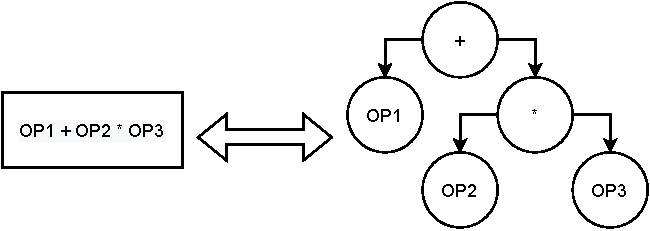
\includegraphics[scale=1.0]{./ressources/expression_to_tree.pdf}
        \caption{Représentation d'une expression arithmétique en arbre binaire}
    \label{fig:exp_arbre}
\end{figure}

\section{Fonctionnement de l'algorithme}
Le passage de l'expression arithmétique en arbre binaire passe par 2 étapes de traduction: l'analyse lexicale et puis la traduction dirigée par la syntaxe (voir Figure \ref{fig:etapes_trad}). L'expression arithmétique est d'abord lue du clavier sous forme de chaîne de caractères. Puis, un vecteur d'entités lexicales est généré à partir de cette chaîne. Enfin, on génère un arbre binaire à partir du vecteur d'entités lexicales.

\begin{figure}[H]
    \centering
        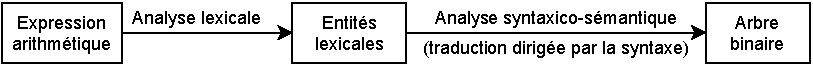
\includegraphics[scale=1.0]{./ressources/translation_steps.pdf}
        \caption{Les étapes de la traduction}
    \label{fig:etapes_trad}
\end{figure}
\par
Les structures de données utilisées dans les algorithmes qui vont suivre sont les suivantes :
\begin{description}
    \item[entité] : représente une entité lexicale et contient les champs type de l'entité et la valeur.     
    \item[noeud] : représente un élément d'un arbre et contient une valeur et des pointeurs vers les fils droit et gauche du noeud.
    \item[arbre] : représente un arbre binaire et contient un pointeur vers la racine de l'arbre.
\end{description}

\subsection{Analyse lexicale}
Dans cette partie, on extrait les entités lexicales de la chaîne de caractères contenant l'expression arithmétique.
On parcourt la chaîne de caractères depuis le début, et on génère les entités lexicales selon les caractères lus.

\begin{algorithm}[H]
    \SetAlgoLined
    \KwData{expression : chaîne de caractères}
    \KwResult{entites : vecteur d'entités}
    \textbf{Variables :}\\
    e : entité\;
    i, j : entier\;
    \Begin{
        Initialiser le vecteur entites à vide\;
        \For{$i \leftarrow 1$\KwTo$expression.taille()$}{
            \uIf{expression[i] est un opérateur}{
                \tcp{Reconnaitre un opérateur}
                e.type$\leftarrow$opérateur\;
                e.operation$\leftarrow$type\_opération\;
                entites.ajouter(e)\;
            }
            \uElseIf{expression[i] est une parenthèse}{
                \tcp{Reconnaitre une parenthèse}
                e.type$\leftarrow$parenthèse\;
                e.parenthèse$\leftarrow$type\_parenthèse\;
                entites.ajouter(e)\;
            }
            \uElseIf{expression[i] est un chiffre ou un point}{
                \tcp{Reconnaitre un nombre}
                j$\leftarrow$1\; 
                \lWhile{$i+j \leq expression.taille()$ et expression[i] est un chiffre ou un point}{j$\leftarrow$$j+1$}
                e.type$\leftarrow$nombre\;
                e.nombre$\leftarrow$en\_nombre(expression.sous\_chaine(i, j))\;
                entites.ajouter(e)\;
                i$\leftarrow$$i+j-1$\;
            }
            \Else{
                Lever une exception\tcp*{Erreur lexicale}
            }
        }
    }
    \caption{Analyse lexicale}
\end{algorithm}

\subsection{Analyse syntaxico-sémantique ou traduction dirigée par la syntaxe}
Nous utilisons l'algorithme de descente récursive pour parcourir le vecteur d'entités et générer l'arbre binaire. Dans cet algorithme chaque MGP (membre de gauche de production) est associé à une fonction dans le programme. L'algorithme commence en appelant une première fois l'axiome de la grammaire et se termine une fois que tout le vecteur est parcouru.
\par
La grammaire utilisée est comme suit :
$$ E \rightarrow T + \{ T \}^* | T - \{ T \}^* $$
$$ T \rightarrow F * \{ F \}^* | F / \{ F \}^* $$
$$ F \rightarrow nb | ( E ) | + F | - F $$

\begin{algorithm}[H]
    \SetAlgoLined
    \KwData{expression : chaîne de caractères}
    \KwResult{entites : vecteur d'entités}
    \textbf{Variables :}\\
    tc : entier\;
    bt : arbre\;
    \Begin{
        ct$\leftarrow$0\;
        \lIf{$tc = entites.taille()$}{Lever une exception\tcp*[f]{Expression vide}}
        bt$\leftarrow$e(entites, tc)\tcp*{Appel de la fonction e}
        \KwRet{bt};
    }
    \caption{Descente récursive}
\end{algorithm}

\par
Cette fonction $e$ traite les opérations d'addition et de soustraction qui sont moins prioritaires, et génère les noeuds correspondants. Le traitement des autres opérations est délégué à la fonction $t$ qui va terminer son exécution avant la fonction $e$; c-à-d. que les noeuds générés par les opérations plus prioritaires seront retournés à la fonction $e$ qui va les ajouter dans les niveaux plus bas.\\
\begin{function}[H]
    \textbf{Variable :}\\
    bt, rt, lt : arbre\;
    e : entité\;
    \Begin{
        bt$\leftarrow$t(entites, tc)\tcp*{Appel de la fonction t}
        \While{$tc \leq entites.taille()$ et entites[tc] est un opérateur d'addition ou de soustraction}{
            e$\leftarrow$entites[tc]\;
            lt$\leftarrow$bt\;
            tc$\leftarrow$tc + 1\;
            \lIf{$tc > entites.taille()$}{Lever une exception\tcp*[f]{Erreur syntaxique}}
            rt$\leftarrow$t(entites, tc)\tcp*{Appel de la fonction t}
            bt.racine$\leftarrow$e\;
            bt.fils\_gauche$\leftarrow$lt\;
            bt.fils\_droit$\leftarrow$rt\;
        }
        \KwRet{bt}\;
    }
    \caption{e(entites : vecteur d'entités, Entrée/Sortie tc : entier) : arbre}
\end{function}

\par
Cette fonction $t$ traite les opérations de multiplication, de division et de modulo. Elle utilise la fonction $f$ pour générer les noeuds des nombres et des sous-expressions plus prioritaires comme les parenthèses.\\
\begin{function}[H]
    \textbf{Variable :}\\
    bt, rt, lt : arbre\;
    e : entité\;
    \Begin{
        bt$\leftarrow$f(entites, tc)\tcp*{Appel de la fonction f}
        \While{$tc \leq entites.taille()$ et entites[tc] est un opérateur de multiplication ou de division ou de modulo}{
            e$\leftarrow$entites[tc]\;
            lt$\leftarrow$bt\;
            tc$\leftarrow$tc + 1\;
            \lIf{$tc > entites.taille()$}{Lever une exception\tcp*[f]{Erreur syntaxique}}
            rt$\leftarrow$f(entites, tc)\tcp*{Appel de la fonction f}
            bt.racine$\leftarrow$e\;
            bt.fils\_gauche$\leftarrow$lt\;
            bt.fils\_droit$\leftarrow$rt\;
        }
        \KwRet{bt}\;
    }
    \caption{t(entites : vecteur d'entités, Entrée/Sortie tc : entier) : arbre}
\end{function}

\par
Cette fonction $f$ génère les noeuds des nombres et des opérateurs unaires, elle repasse le contrôle à la fonction $e$ en cas d'utilisation de parenthèses pour traiter la sous-expression contenue dedans.\\
\begin{function}[H]
    \textbf{Variable :}\\
    bt, rt, lt : arbre\;
    e, gauche, droit : entité\;
    \Begin{
        \uIf{entites[tc] est une parenthèse ouvrante}{
            tc$\leftarrow$tc + 1\;
            \lIf{$tc > entites.taille()$}{Lever une exception\tcp*[f]{Erreur syntaxique}}
            bt$\leftarrow$e(entites, tc)\tcp*{Appel de la fonction e}
            \uIf{$tc \leq entites.taille()$ et entites[tc] est une parenthèse fermante}{
                tc$\leftarrow$tc + 1\;
            }
            \Else{
                Lever une exception\tcp*[f]{Erreur Syntaxique}
            }
        }
        \uElseIf{entites[tc] est un opérateur d'addition ou de soustraction}{
            \tcp{Cas d'un opérateur unaire}
            e$\leftarrow$entites[ct]\;
            gauche.type$\leftarrow$type\_nombre\;
            gauche.nombre$\leftarrow$0\;
            tc$\leftarrow$tc + 1\;
            \lIf{$tc > entites.taille()$}{Lever une exception\tcp*[f]{Erreur syntaxique}}
            rt$\leftarrow$f(entites, tc)\tcp*{Appel de la fonction f}
            lt.racine$\leftarrow$gauche\;
            bt.racine$\leftarrow$e\;
            bt.fils\_gauche$\leftarrow$lt\;
            bt.fils\_droit$\leftarrow$rt\;
        }\Else{
            \tcp{Cas d'un nombre (feuille de l'arbre)}
            e$\leftarrow$entites[tc]\;
            bt.racine$\leftarrow$e\;
            tc$\leftarrow$tc + 1\;
        }
        \KwRet{bt}\;
    }
    \caption{f(entites : vecteur d'entités, Entrée/Sortie tc : entier) : arbre}
\end{function}

\section{Calcul de complexité}
\subsection{Complexité temporelle}
La complexité de l'analyse lexicale est toujours égale à la longueur de la chaîne dans tous les cas c-à-d. : $\mathcal{O}(n)$ tel que $n$ est la longueur de l'expression en de caractères.
\par
La complexité de l'analyse syntaxique est quant à elle égale à la longueur du vecteur d'entités lexicales, car il est parcouru une seule fois, c-à-d. : $\mathcal{O}(n')$ tel que $n'$ est la longueur du vecteur d'entités.
\par
La complexité temporelle de l'algorithme devient alors : $\mathcal{O}(n + n')$. Sachant que $n > n'$ (le nombre de caractères est supérieur au nombre d'opérandes) on peut remplacer $n'$ par $n$, et la formule devient : $\mathcal{O}(n)$ qui est une complexité linéraire.

Le tableau suivant représente les temps d'exécution théorique en nanoseconde de l'algorithme selon la variation de la taille de l'expression:

\small
\begin{center}
\begin{tabular}{| c | c | c | c | c | c | c | c | c | c | c | c | c |}
    \hline
    N & 10 & 50 & 100 & 500 & 1000 & 5000 & 10000 & 100000 & 1000000 & 10000000 \\
    \hline
    t(ns) & 10 & 50 & 100 & 500 & 1000 & 5000 & 10000 & 100000 & 1000000 & 10000000 \\
    \hline
\end{tabular}  
\end{center}

La figure suivante (voir Figure \ref{fig:temps_exec_th_algo2}) représente l'évolution du temps d'exécution théorique selon la longueur de l'expression.

\begin{figure}[H]
    \centering
        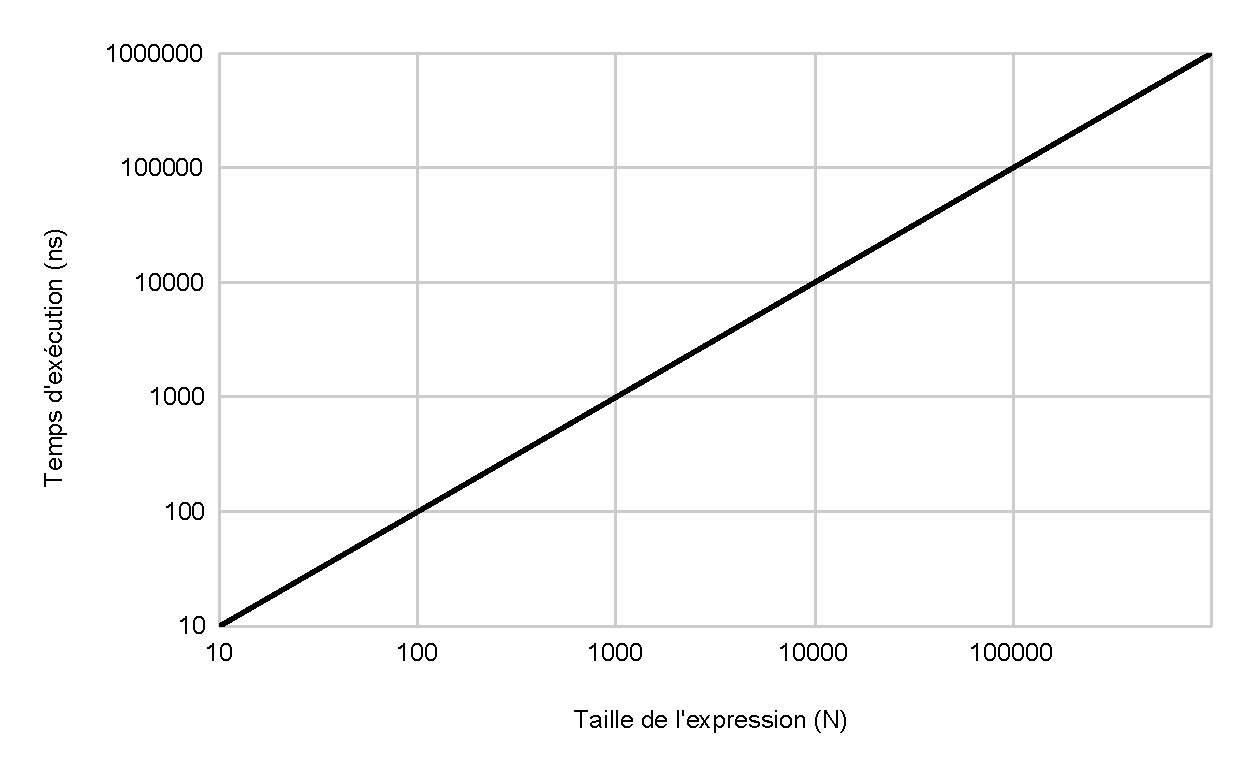
\includegraphics[scale=0.5]{./ressources/temps_execution_th_algo2.pdf}
        \caption{Temps d'exécution théorique de l'algorithme de représentation d'expression arithmétique en arbre binaire}
    \label{fig:temps_exec_th_algo2}
\end{figure} 

Depuis le graphe,  on observe que le temps d'exécution évolue de manière linéaire avec l'évolution de la taille de l'expression.

\subsection{Complexité spatiale}
L'expression arithmétique est d'abord stockée dans une chaîne de caractères de longueur $n$, puis dans un vecteur d'entités de longueur $n'$, puis dans un arbre binaire qui contient lui aussi $n'$ éléments.
\par
Sachant qu'une entité contient le type de l'entité et la valeur en elle-même, cependant la valeur est stockée comme un nombre réel qui prend 8 octets comparé à la représentation en chaîne de caractères où chaque caractère est sous 1 octet.
\par
Donc la taille d'un élément d'une chaîne de caractères est $1$ unité (octet), la taille d'une entité est $9$ unités, et la taille d'un élément d'un arbre est égale à $9 + 4 * 2$ unités (la taille d'un pointeur est égale à $4$ unités) donc $17$ unités.
\par
La complexité spatiale est égale à la somme des trois complexités (taille de la chaîne + taille du vecteur + taille de l'arbre) : $n * 1 + n' * 9 + n' * 17 = n + n' * 26 \approx \mathcal{O}(n + n')$
\par

\section{Expérimentation}
Le tableau suivant représente les temps d'exécution en nanoseconde de l'algorithme selon la variation de la taille de l'expression arithmétique.\\
\small
\begin{tabular}{| c | c | c | c | c | c | c | c | c | c | c | c |}
    \hline
    N &  10 & 50 & 100 & 500 & 1000 & 5000 & 10000 & 100000 & 1000000 \\
    \hline
    t1(ns) & 177584 & 437769 & 381575 & 418252 & 686466 & 3111420 & 6786260 & 60986100 & 642610000 \\
    \hline
    t2(ns) & 101653 & 193648 & 339100 & 354777 & 2322770 & 3307840 & 20424500 & 59967200 & 639145000 \\
    \hline
    t3(ns) & 31972 & 47574 & 216601 & 354751 & 2115200 & 3375350 & 7450650 & 60956700 & 639422000 \\
    \hline
    t4(ns) & 100708 & 149167 & 259485 & 337421 & 820084 & 3283810 & 19698800 & 61631500 & 641354000 \\
    \hline
    t5(ns) & 24343 & 140434 & 95821 & 345987 & 683119 & 5158840 & 7575520 & 61750100 & 640897000 \\
    \hline
    t6(ns) & 30901 & 161277 & 337395 & 807634 & 671850 & 3292160 & 21818400 & 61473700 & 641686000 \\
    \hline
    t7(ns) & 52941 & 140159 & 288308 & 329206 & 693785 & 4360970 & 8418610 & 60870500 & 667895000 \\
    \hline
    t8(ns) & 69185 & 163825 & 242197 & 520649 & 2050330 & 5460620 & 22419800 & 63008000 & 639987000 \\
    \hline
    t9(ns) & 69510 & 97011 & 93270 & 356979 & 692529 & 5279490 & 6420450 & 61725500 & 640873000 \\
    \hline
    t10(ns) & 83819 & 142928 & 92484 & 1071680 & 803473 & 13108600 & 6558390 & 60088300 & 639895000 \\
    \hline
    Moyenne(ns) & 74262 & 167379 & 234624 & 489734 & 1153961 & 4973910 & 12757138 & 61245760 & 643376400 \\
    \hline
\end{tabular}
\normalsize
\par
La figure suivante (voir Figure \ref{fig:temps_exec_algo2}) représente l'évolution du temps d'exécution selon la longueur de l'expression arithmétique.

\begin{figure}[H]
    \centering
        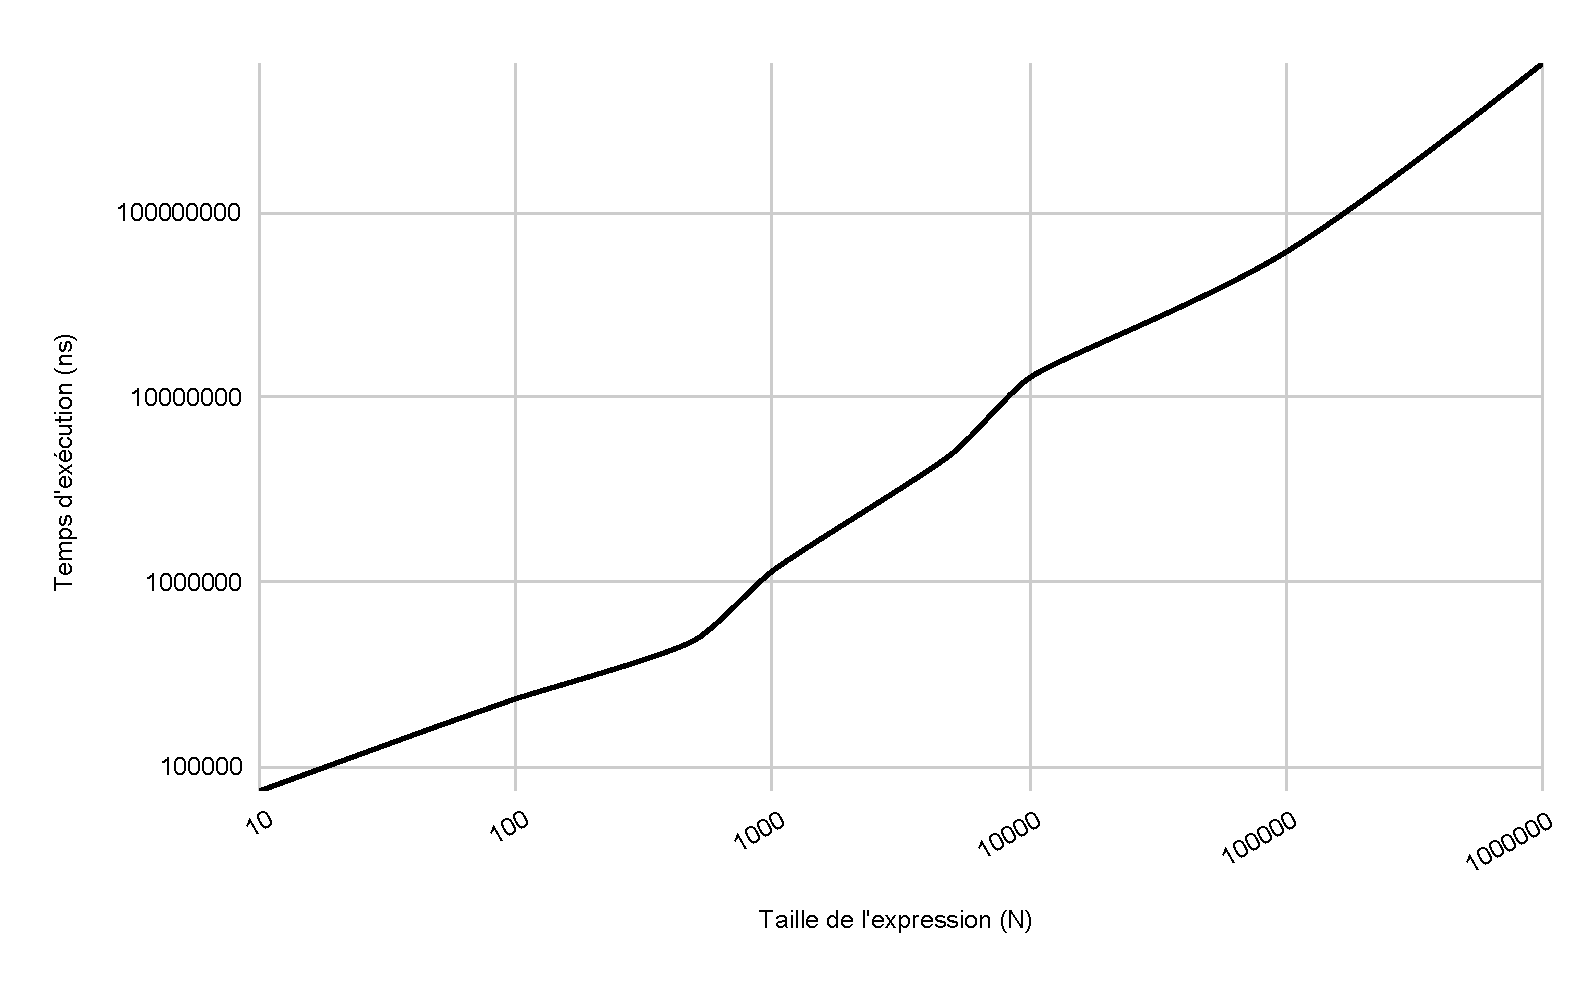
\includegraphics[scale=0.5]{./ressources/temps_execution_algo2.pdf}
        \caption{Temps d'exécution du programme selon la longueur de l'expression}
    \label{fig:temps_exec_algo2}
\end{figure}
\par
Depuis le graphe, la courbe est sous forme d'une droite, on observe que le temps d'exécution évolue de manière linéaire avec l'augmentation de la taille du problème, ce qui correspond bien à la complexité théorique calculée auparavant. 

\section{Améliorations}
Une amélioration possible de l'algorithme consiste à fusionner l'analyse lexicale et syntaxique dans une même itération, c-à-d. que l'entité lexicale est injectée dans l'analyse syntaxique dès qu'elle est reconnue par l'analyse lexicale, sans effectuer une deuxième fois le parcours de l'expression. Cela va diminuer la complexité temporelle de moitié, et la complexité spatiale d'un tier.

\section{Conclusion}
L'algorithme de la descente récursive propose une complexité optimale pour la représentation de l'expression arithmétique en arbre binaire, égale à la longueur de l'expression arithmétique, car il parcourt l'expression un nombre minimal de fois (une seule fois). Nous avons bien vu pendant les expériences que l'évolution du temps d'exécution d'une telle complexité est relativement contrôlé et suit une courbe droite et linéaire.



    \newpage
    \onehalfspacing
    \chapter{Recherche dichotomique d'un élément dans un tableau}

\section{Description de l'objectif de l'algorithme}
En informatique, un tableau est une structure de données représentant une séquence finie d'éléments défini par un index représentant sa position au sein du tableau nous permettant d'y accéder. C'est un type de conteneur que l'on retrouve dans un grand nombre de langages de programmation et est l'un des plus utilisés du de sa simplicité.
\par
Les données du tableau étant accessible individuellement il est nécessaire de faire une recherche lorsque l'on souhaite accéder a une valeur spécifique du tableau cependant lorsque la taille de la structure est grande il devient difficile d'y accéder efficacement, c'est pour cela que de nombreux algorithmes ont été conçu afin d'optimiser cette tache est l'un de ses algorithmes les plus performants est celui de la recherche dichotomique.
\par
La recherche dichotomique ou recherche par dichotomie, est un algorithme de recherche pour trouver la position d'un élément dans un tableau. La seule condition a son application étant que le tableau soit trie, il est utilisable dans de nombreuses problématiques. Son principe consiste comparer l'élément avec la valeur de la case au milieu du tableau, si les valeurs sont égales, on met fin à l'exécution, sinon si la valeur recherchée est inférieur à la valeur de la case au milieu, on recommence dans la moitié du tableau contenant les valeurs plus petites que celle située au milieu du tableau et dans le cas contraire on prend la moitie contenant les valeurs supérieures, et ceci jusqu'à avoir trouvé la valeur souhaite ou avoir un sous tableau n'ayant qu'une seule valeur empêchant de continuer la recherche dans le cas ou la valeur n'existe pas dans le tableau. (voir Figure \ref{fig:exp_dico}).

\begin{figure}[H]
    \centering
        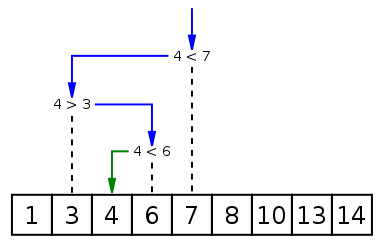
\includegraphics[scale=1.0]{./ressources/Binary_search_into_array.png}
        \caption{Exemple graphique d'une recherche dichotomique}
    \label{fig:exp_dico}
\end{figure}

\section{Fonctionnement de l'algorithme}
Il nous est possible de distinguer 2 étapes distinctes et essentiels au bon déroulement de cet algorithme la première étant le trie du tableau, car comme précisé précédemment la recherche par dichotomie nécessite que le tableau soit trié et ne pouvant pas garantir de recevoir un tableau trié en entrée il est nécessaire de le trier au préalable avant de commencer le recherche afin de pouvoir le plus de cas que possible, par la suite la seconde étape consiste à appliquer la recherche dichotomique.

\subsection{Tri du tableau}
Dans cette partie, on applique un tri ascendant sur tableau et pour cela nous appliquons l'algorithme de Tri Fusion.
\par
Le tri par fusion aussi appeler tri dichotomique est un exemple classique d'algorithme de division pour régner. L'opération principale de l'algorithme est la fusion, qui consiste à réunir deux listes triées en une seule. L'efficacité de l'algorithme vient du fait que deux listes triées peuvent être fusionnées en temps linéaire (voir Figure \ref{fig:tri_dico}). On peut résumer son fonctionnement en deux étapes :
\begin{enumerate}
  \item Divisez la liste non triée en sous-listes jusqu'à ce qu'il y ait N sous-listes avec un élément dans chacune (N est le nombre d'éléments dans la liste non triée).
  \item Fusionnez les sous-listes deux à la fois pour produire une sous-liste triée, répétez cette opération jusqu'à ce que tous les éléments soient inclus dans une seule liste.
\end{enumerate}

\begin{figure}[H]
    \centering
        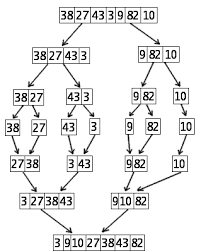
\includegraphics[scale=1.0]{./ressources/trifusion.png}
        \caption{Exemple graphique d'un tri dichotomique}
    \label{fig:tri_dico}
\end{figure}
\par
Nous pouvons le représenter via le pseudo code suivant :

\begin{function}[H]
    \textbf{Variables :}\\
    TabG, TabD : tableau d'entier\;
    SousTab1, SousTab2, SousTab1Index, SousTab2Index, SousTabFusionIndex : entier\;
    \Begin{
        $SousTab1  \leftarrow milieu - gauche + 1$\;
        $SousTab2  \leftarrow droite - milieu$\;
        \For{$i \leftarrow 1$ \KwTo $SousTab1$}{
            $tabG[i] \leftarrow tab[gauche + i]$\;
        }
        \For{$j \leftarrow 1$ \KwTo $SousTab2$}{
            $tabG[j] \leftarrow tab[mid + 1 + j]$\;
        }
        $SousTab1  \leftarrow 0$\;
        $SousTab2  \leftarrow 0$\;
        $SousTabFusionIndex  \leftarrow gauche$\;
        \While{$SousTab1Index < SousTab1$ et $SousTab2Index < SousTab2$}
       {
            %\\
            \uIf{tabG[SousTab1Index] <= tabD[SousTab2Index]}{
                $tab[SousTabFusionIndex] \leftarrow tabG[SousTab2Index]$\;
                $SousTab1Index++$\;
            }
            \Else {
                $tab[SousTabFusionIndex] \leftarrow tabD[SousTab2Index]$\;
                $SousTab2Index++$\;
            }
            $SousTabFusionIndex++$\;
        %\EndWhile
        }
        \While{$SousTab1Index < SousTab1$}
       {
            %\\
            $tab[SousTabFusionIndex] \leftarrow tabG[SousTab1Index]$\;
            $SousTab1Index++$\;
            $SousTabFusionIndex++$\;
        %\EndWhile
        }
        \While{$SousTab2Index < SousTab2$}
       {
            %\\
            $tab[SousTabFusionIndex] \leftarrow tabG[SousTab2Index]$\;
            $SousTab1Index++$\;
            $SousTabFusionIndex++$\;
        %\EndWhile
        }
    }
    \caption{Fusion(Entrée: tab: tableau d'entier; droite, gauche, milieu: entier;)}
\end{function}

\begin{function}[H]
    \textbf{Variables :}\\
    milieu : entier\;
    \Begin{
        \tcp{On divive le tableau en 2 de manière recursive puis on les tri avant de les fusionner}
        \If{$debut >= fin$}
            {retour\;}
        \tcp{On calcule l'index du milieu du tableau}
        $milieu \leftarrow debut + (fin - debut) / 2$\;
        TriFusion(tab, debut, milieu)\;
        TriFusion(tab, milieu + 1, fin)\;
        \tcp{On utilise la fonction fusion pour trier puis fusioner les sous tableaux en un seul tableau trié}
        Fusion(tab, debut, mid, fin)\;
    }
    \caption{TriFusion(Entrée: tab: tableau d'entier; debut, fin: entier;)}
\end{function}
\par
Afin d'optimiser le déroulement du tri, nous utilisons 2 fonctions distinctes. Une fonction TriFusion qui divise le tableau récursivement et une fonction Fusion qui elle trie les sous tableaux avant de les fusionner à nouveau
\subsection{Recherche dichotomique}
La recherche dichotomique consiste à rechercher dans un tableau trié en divisant l'intervalle de recherche en deux.
On commence par un intervalle couvrant tout le tableau. Si la valeur de la clé de recherche est inférieure à l'élément situé au milieu de l'intervalle, on limite l'intervalle à la moitié inférieure. Sinon, le réduire à la moitié supérieure. On vérifie à plusieurs reprises jusqu'à ce que la valeur soit trouvée ou que l'intervalle soit vide.
\par
Nous pouvons le représenter via le pseudo code suivant :

\begin{function}[H]
    \textbf{Variables :}\\
    debut, fin, milieu : entier\;
    \Begin{
    \tcp{si la valeur recherchée est superieur ou inferieur au bornes du tableau on retourne -1 si elle est égale a une des bornes on retourn leur positions}
        \If{$r < tab[0]$ ou $r > tab[n-1]=$}
            {$pos \leftarrow -1$\;
             retour pos\;}
        \If{$tab[0] == r$}
            {$pos \leftarrow 0$\;
             retour pos\;}
        \If{$tab[n-1] == r$}
            {$pos \leftarrow n - 1$\;
             retour pos\;}
        \While {$fin >= debut$}
        {
            \tcp{Calcul de la position de l'élément du milieu}
            $i \leftarrow (debut + fin) / 2$\;
            \tcp{Si l'élément du milieu est l'élément recherché on retourne sa position}
            \uIf{$tab[i] == r$}
                {$pos \leftarrow i$\;
                 retour pos\;}
            \tcp{Si la valeur recherchée est plus petite que la valeur du l'élément du milieu Alors on regarde le sous-tableau de gauche}
            \uElseIf {$tab[i] > r$}
                {$fin = i - 1$\;}
            \tcp{sinon on regarde le sous-tableau de droite}
            \Else
                {$debut = i + 1$\;}
        }
    }
    \caption{dichotomie(Entrée: tab: tableau d'entier; n, r: entier; Sortie: pos)}
\end{function}

\section{Calcul de complexité}
\subsection{Complexité temporelle}
La complexité du tri dichotomique est toujours égale à : $\mathcal{O}(n \log(n))$ que ce soit dans le cas meilleur ou le cas tel que $n$ est la longueur du tableau.
\par
La complexité de la recherche dichotomique  est quant à elle égale à $\mathcal{O}(\log(n'))$ tel que $n'$ est la longueur du tableau.
\par
La complexité temporelle de l'algorithme devient alors : $\mathcal{O}(n \log(n) + \log(n')) = {O}(\log(n^n + n'))$.\\

Le tableau suivant représente les temps d'exécution théorique en nanoseconde de l'algorithme selon la variation de la taille du tableau

\small
\begin{center}
\begin{tabular}{| c | c | c | c | c | c | c | c | c | c | c | c | c |}
    \hline
    N &  10 & 50 & 100 & 500 & 1000 & 5000 & 10000 & 100000 & 1000000 & 10000000 \\
    \hline
    t(ns) & 11 & 87 & 202 & 1352 & 3003 & 18499 & 40004 & 500005 & 6000006 & 70000007 \\
    \hline
\end{tabular}  
\end{center}

La figure suivante (voir Figure \ref{fig:temps_exec_dico_theo}) représente l'évolution du temps d'exécution théorique selon la longueur du tableau.

\begin{figure}[H]
    \centering
        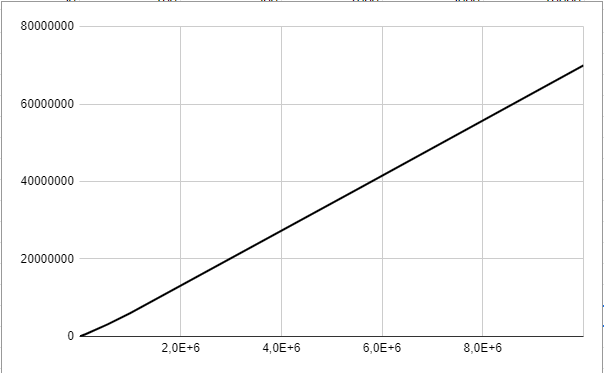
\includegraphics[scale=0.5]{./ressources/tempsexecutiondicotheorique.png}
        \caption{Temps d'exécution théorique du programme selon la longueur du tableau}
    \label{fig:temps_exec_dico_theo}
\end{figure} 

Depuis le graphe,  on observe que le temps d'exécution évolue de manière linéarithmique avec l'augmentation de la taille du problème.

\subsection{Complexité spatiale}
L'expression arithmétique est d'abord stockée dans une chaîne de caractères de longueur $n$, puis dans un vecteur d'entités de longueur $n'$, puis dans un arbre binaire qui contient lui aussi $n'$ éléments.
\par
L'unique structure de données utilisée est un tableau d'entier a n éléments. 
\par
La taille d'un entier étant de 2 octets la complexité spatiale est égale au produit de la taille du tableau et de la taille d'un entier : $n * 2 \approx \mathcal{O}(n)$
\par

\section{Expérimentation}
Le tableau suivant représente les temps d'exécution expérimentale en nanoseconde de l'algorithme selon la variation de la taille du tableau.

\small
\begin{center}
\resizebox{19cm}{!}{
\begin{tabular}{| c | c | c | c | c | c | c | c | c | c | c | c | c |}
    \hline
    N &  10 & 50 & 100 & 500 & 1000 & 5000 & 10000 & 100000 & 1000000 & 10000000 \\
    \hline
    t1(ns) & 2164 & 28704 & 92760 & 169733 & 341583 & 1047560 & 4598740 & 35465600 & 5626090000 & 37018600000 \\
    \hline
    t2(ns) & 6674 & 35401 & 75401 & 251223 & 600691 & 1642120 & 3621170 & 34767200 & 3774520000 & 33572800000 \\
    \hline
    t3(ns) & 5654 & 33403 & 53403 & 275397 & 771243 & 1225350 & 2874540 & 40542400 & 2998740000 & 36542700000 \\
    \hline
    t4(ns) & 4233 & 42553 & 82553 & 251567 & 477149 & 988353 & 4714569 & 37218300 & 3411720000 & 36325400000 \\
    \hline
    t5(ns) & 5904 & 58861 & 58861 & 163133 & 348047 & 1253250 & 3148226 & 37992800 & 3845760000 & 29451700000 \\
    \hline
    t6(ns) & 5645 & 20634 & 70634 & 252684 & 801493 & 1991560 & 2132380 & 40874100 & 298370000 & 401745900000 \\
    \hline
    t7(ns) & 3820 & 43164 & 64307 & 251082 & 481145 & 1035130 & 3258380 & 37476600 & 3220570000 & 36945100000 \\
    \hline
    t8(ns) & 5641 & 32783 & 57953 & 283887 & 428472 & 2290770 & 2811460 & 28514100 & 3859450000 & 28416500000 \\
    \hline
    t9(ns) & 7242 & 47059 & 65421 & 258297 & 429683  & 1988180 & 3223750 & 3589600 & 3042580000 & 35473800000 \\
    \hline
    t10(ns) & 5242 & 31262 & 41654 & 233613 & 530896 & 1041460 & 3706200 & 45122700 & 1687400000 & 33447800000 \\
    \hline
    Moyenne(ns) & 5221 & 37382 & 66294 & 239061 & 521040 & 1271437 & 3429518 & 37552644 & 3176520000 & 70894030000 \\
    \hline
\end{tabular}}
\end{center}
\normalsize
\par
La figure suivante (voir Figure \ref{fig:temps_exec_dico}) représente l'évolution du temps d'exécution selon la longueur du tableau.

\begin{figure}[H]
    \centering
        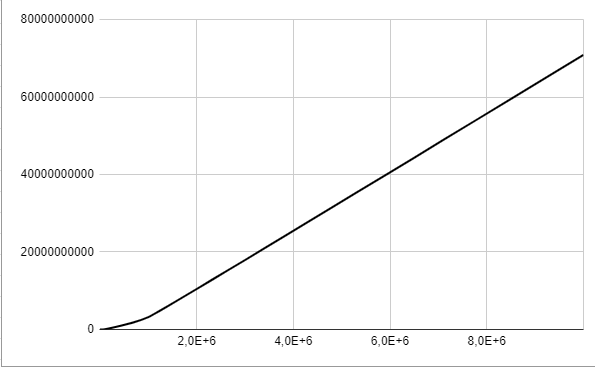
\includegraphics[scale=0.55]{./ressources/tempsexecutiondico.png}
        \caption{Temps d'exécution du programme selon la longueur du tableau}
    \label{fig:temps_exec_dico}
\end{figure}

\par
Depuis le graphe,  on observe que le temps d'exécution évolue de manière linéarithmique avec l'augmentation de la taille du problème, ce qui correspond bien à la complexité théorique et d’exécution théorique calculée auparavant. 

\section{Conclusion}
L'algorithme de la recherche dichotomique propose une complexité optimale pour la recherche dans un tableau, cependant sa dépendance d'une fonction de tri afin de pouvoir fonctionner Quel que soit le tableau donné impacte négativement sa complexité, dans notre l'utilisation d'une fonction de tri dichotomique aura fait passer notre algorithme d'une complexité logarithmique a une complexité linéarithmique. Nous pouvons en conclure que la recherche par dichotomie est effectivement une bonne option, mais qu'afin de pouvoir l'utiliser à son plein potentiel il est nécessaire de l'utiliser sur des tableaux préalablement triés ou accompagné d'une fonction de tri ayant une complexité égale ou meilleure à elle.


    \newpage
    \onehalfspacing
    \chapter{Suppression d'un élément dans un arbre binaire de recherche}

\section{Description de l'objectif de l'algorithme}
Les arbres binaires représentent une structure de données très utilisée pour effectuer des tâches en informatique, d’une part parce que ce type de données permet de stocker des données volumineuses facilement accessibles, et d’autre part, les informations sont souvent hiérarchisées, et peuvent être représentées naturellement sous une forme arborescente.
\par
Un arbre est un ensemble organisé de nœuds dans lequel chaque nœud a un seul père, à l’exception de la racine qui est un nœud sans père. 
\par
 Si le nœud p est le père du nœud f, nous dirons que f est un fils de p, et si le nœud p n’a pas de fils nous dirons que c’est une feuille. Chaque nœud porte une valeur (également appelée clé ou étiquette) et deux pointeurs, un qui pointe son fils gauche et l’autre sur le droit.  
 \par
 Un arbre binaire de recherche (ABR) est un arbre qui permet de représenter un ensemble de valeurs ayant une relation d’ordre.C'est à dire que pour tout nœud de cet arbre, sa valeur est strictement plus grande que les valeurs figurant dans son sous-arbre gauche et strictement plus petite que les valeurs figurant dans son sous-arbre droit. Cela implique qu’une valeur n’apparaît au plus qu’une seule fois dans un arbre de recherche.(voir Figure \ref{fig:arb}).
 \par
 Les opérations caractéristiques sur les arbres binaires de recherche sont l’insertion, la suppression, et la recherche d’une valeur. Le cout de ces dernières dépend du degré d’équilibre de l’arbre. 
 \par 
 La suppression d'un élèment dans un arbre binaire de recherche est une opération compliquée. En effet, on doit d'abord trouver le noeud, le supprimer, ensuite nous devons faire le nécessaire pour conserver la structure de l'arbre.  

\begin{figure}[H]
    \centering
        
\includegraphics[scale=0.2]{./ressources/arbre.png}
        \caption{Exemple graphique d'un arbre binaire de recherche}
    \label{fig:arb}
\end{figure}

\section{Fonctionnement de l'algorithme}
L’opération de suppression d’un nœud dépend du nombre de ses fils dans l’arbre. Les différents cas de figure possibles sont les suivants

\subsection{Cas 1 : Cas d’une feuille. Le nœud à supprimer n’a pas de fils}
Il suffit d'enlever le nœud en modifiant le lien du père, s’il existe. Sinon l'arbre devient un arbre vide.  (voir Figure \ref{fig:d1}).
\begin{figure}[H]
    \centering
        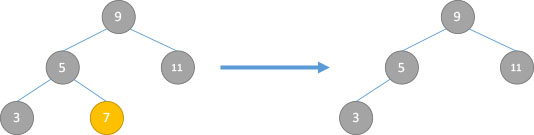
\includegraphics[scale=0.8]{./ressources/d1.jpeg}
        \caption{Exemple de suppression d'une feuille}
    \label{fig:d1}
\end{figure}

\subsection{Cas 2 : Cas d’un unique fils Le nœud à supprimer à un unique fils}
On décroche le noeud de l’arbre comme dans le cas 1.Ensuite,on relie directement son père et son fils. Si ce père n’existe pas, l’arbre est réduit au fils unique du nœud supprimé.  (voir Figure \ref{fig:d2}).
\begin{figure}[H]
    \centering
        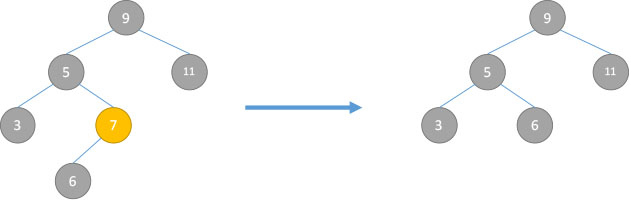
\includegraphics[scale=0.7]{./ressources/d2.jpeg}
        \caption{Exemple de suppression d'un noeud à un seul fils}
    \label{fig:d2}
\end{figure}

\subsection{Cas 3 : Cas de deux fils Le nœud à supprimer à deux fils}
On cherche le successeur en ordre du noeud. Ensuite, on copie le contenu du successeur d'ordre dans le noeud et on supprime le successeur d'ordre. Notez que le prédécesseur d'ordre peut également être utilisé.
\par
Il est important de noter que le successeur d'ordre peut être obtenu en trouvant la valeur minimale dans le sous-arbre de droite du noeud à supprimer et que le prédécesseur d'ordre est le maximum de son sous-arbre gauche.(voir Figure \ref{fig:d3}).
\begin{figure}[H]
    \centering
        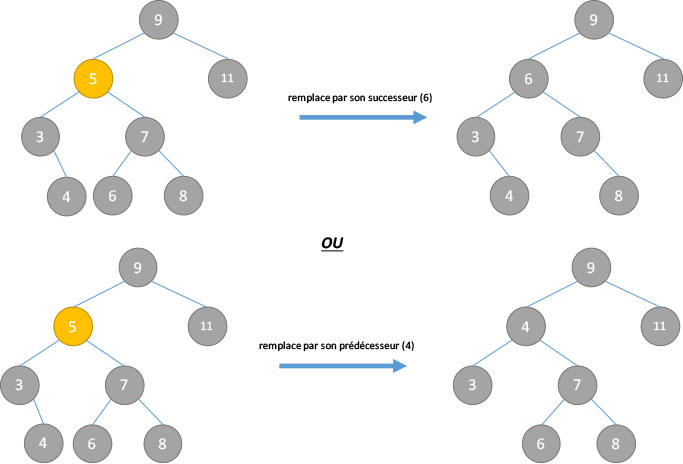
\includegraphics[scale=0.6]{./ressources/d3.jpeg}
        \caption{Exemple de suppression d'un noeud à deux fils}
    \label{fig:d3}
\end{figure}
\par


\begin{function}[H]
    \textbf{Variables :}\\
    Temp: arbre\;
    \Begin{
        \If{$racine = Nil$}
            {retour Nil\;}
        \ENDIF
        \If{$valeur < racine.valeur$}{
            \tcp{Si la valeur cherchée est inférieure à l'élèment en cours, on supprime à gauche}
            $racine.filsg \leftarrow supprimerec(racine.filsg, valeur)$\;}
        \Elseif{$valeur > racine.valeur$}{
        \tcp{Si la valeur cherchée est supérieure à l'élèment en cours, on supprime à droite}
            $racine.filsd \leftarrow supprimerec(racine.filsd, valeur)$\;}
        \Else
        {
        \tcp{Si la valeur est trouvée, on distigue 3 cas}
        \tcp{Le noeud n'a pas de fils}
        \If{$racine.filsg = Nil$ et $racine.filsd = Nil$}{
        retour Nil\;}
        \Elseif{$racine.filsd = Nil$}
        {
        \tcp{Si le noeud a un fils gauche seulement}
        $Temp \leftarrow racine.filsg$ \;
        Libérer(racine)\;
        retour Temp \;
        }
        \Elseif{$racine.filsg = Nil$}{
        \tcp{Si le noeud a un fils à droite seulement}
        $Temp \leftarrow racine.filsd$ \;
        Libérer(racine)\;
        retour Temp \;
        }
        
        $Temp \leftarrow Min(racine.filsd)$\; \tcp{Peut etre remplacé par $Temp \leftarrow Max(racine.filsg)$\;}
        $racine.valeur \leftarrow Temp.valeur$ \;
        $racine.filsd \leftarrow supprimerec(racine.filsd, Temp.valeur)$ \; \tcp{Peut etre remplacé par $racine.filsg \leftarrow supprimerec(racine.filsg, Temp.valeur)$ \;}
        }
        \ENDIF
        retour racine;
    }
    \caption{supprimerec(Entrée: racine: arbre, valeur: entier) : arbre}
\end{function}
\par 
Comme nous l'avons mentionné avant, quand on veut supprimer un nœud qui a deux fils, nous devons écraser sa valeur en optant pour l’une des deux options : soit on cherche le successeur en ordre du nœud à supprimer, soit son prédécesseur en ordre. Il est à noter que le successeur en ordre du nœud représente le minimum dans son sous-arbre à droite, et que son prédécesseur représente le maximum de son sous-arbre gauche. Voici donc les deux fonctions que nous pourrons utiliser pour effectuer ces deux tâches :
\par
\begin{function}[H]
    \textbf{Variables :}\\
    min: arbre\;
    \Begin{
    $min \leftarrow racine$ \;
        \While{$min <> Nil$ et $min.filsg <> Nil$}{
        $ min \leftarrow min.filsg$ \;
       }
       retour min;
    }
    \caption{Min(Entrée: racine: arbre) : arbre}
\end{function}

\begin{function}[H]
    \textbf{Variables :}\\
    max: arbre\;
    \Begin{
    $max \leftarrow racine$ \;
        \While{$max <> Nil$ et $max.filsd <> Nil$}{
        $ max \leftarrow max.filsd$ \;
       }
       retour max;
    }
    \caption{Max(Entrée: racine: arbre) : arbre}
\end{function}

\par 
Puisque l’opération de suppression est une tâche complexe, nous avons, en premier lieu opter pour la méthode récursive. Celle-ci nous permet d’avoir une vue globale sur les cas auxquels nous pourrons être confrontés et comment procéder pour garder la structure de l’arbre intacte même après la suppression.  
\par
Maintenant, nous allons écrire l’algorithme itératif de suppression pour comprendre comment s’effectue la suppression en détail. 

\begin{function}[H]
    \textbf{Variables :}\\
    Temp, actuel, min, pere, prec: arbre\;
    \Begin{
    $actuel \leftarrow racine$ \;
    $prec \leftarrow Nil$ \;
        \While{$actuel <> Nil$ et $actuel.valeur <> valeur$}{
        $ prec \leftarrow actuel$ \;
        \If{valeur < actuel.valeur}{
        $actuel \leftarrow actuel.filsg$\;
        \Else{$actuel \leftarrow actuel.filsd$\;}
        }
        }
        \If{$actuel = Nil$}{
        Ecrire("La valeur que vous voulez supprimer n'existe pas dans l'arbre")\;
        retour racine\;
        }
        \If{$actuel.filsg = Nil$ ou $actuel.filsd = Nil$}{ \tcp{Si le noeud a au plus un fils}
        \If{$actuel.filsg = Nil$}{ 
        $Temp \leftarrow actuel.filsd$\;
        }
        \Else{$Temp \leftarrow actuel.filsg$\;}
        \If{$prec = Nil$}{ \tcp{Si le noeud est une racine}
        retour Temp\;
        }
        \If{actuel = prec.filsd}{ \tcp{Si le noeud est une fils à droite}
        prec.filsd = Temp\;
        }
        \Else{prec.filsg = Temp\;}
        Libérer(actuel)\;
        }
    }
    \caption{supprimeiter(Entrée: racine: arbre, valeur: entier) : arbre}
\end{function}



\begin{function}[H]

     \Else{ \tcp{Si le noeud à supprimer a deux fils}
        \tcp{On commence par chercher le successeur en ordre}
        $Temp \leftarrow actuel.filsd$\;
        $pere \leftarrow racine$\;
        \While{$Temp.filsg <> Nil$}{
        $pere \leftarrow Temp$\;
        $Temp \leftarrow Temp.filsg$\;
        }
        \If{$pere <> racine$}{
        \tcp{On peut mettre fils droit du successeur comme fils gauche du père du successeur }
        $pere.filsg \leftarrow Temp.filsd$\;
        }
        \Else{
        $actuel.filsd \leftarrow temp.filsd$\;
        }
        $actuel.valeur \leftarrow Temp.valeur$\; \\
        Libérer(Temp)\;
        }
        retour racine\;
    \caption{supprimeiter(Entrée: racine: arbre, valeur: entier) : arbre}
\end{function}


\section{Calcul de complexité}
\subsection{Complexité temporelle}
Dans le meilleur cas, nous aurons un ABR équilibré, c’est-à-dire que le nombre des fils à gauche est le même qu’à la droite. La complexité temporelle est donc de l’ordre de la hauteur de l’arbre binaire de recherche. Puisque ce dernier est en moyenne $\mathcal{O}(log_2(n)$, la complexité temporelle du cas moyen est de l’ordre $\mathcal{O}(log_2(n)$. Il en va de même pour le cas moyen.
\par
Nous avons obtenu une complexité temporelle logarithmique parce que la suppression dans un arbre binaire de recherche est un cas où un problème de taille n est divisé en sous-problèmes de taille n/2 jusqu'à atteindre un problème de taille 1.
\par
Le calcul de la complexité se fait donc de la manière suivante :
$$ \frac {a}{b^x}=1  \hspace{2cm}[Dans\hspace{0.2cm} un\hspace{0.2cm} arbre\hspace{0.2cm} binaire\hspace{0.2cm} b = 2] $$
$$i.e : n=2^x\hspace{2cm} qui\hspace{0.2cm} est\hspace{0.2cm} log_2 n\hspace{0.2cm} par\hspace{0.2cm} definition\hspace{0.2cm} de\hspace{0.2cm} la\hspace{0.2cm} fonction\hspace{0.2cm} logarithme$$

\par
Par ailleurs, si on traverse de la racine à une feuille, c’est-à-dire toute la hauteur $h$ de l’arbre. Si ce dernier n’est pas équilibré, on sera amené à parcourir tous les nœuds et la hauteur de l’arbre deviendra $n$. par conséquent la complexité temporelle dans le pire des cas de l’opération de suppression est $\mathcal{O}(n)$.


\subsection{Complexité spatiale}

\par
Nos noeuds sont directement stockées dans un arbre de recherche à $n$ éléments. Dans notre cas, une entité contient une valeur entière et deux pointeurs pour les deux fils. La taille de la valeur stockée ainsi qu'un pointeur fait 4 octets. Donc la taille d'un élèment dans l'arbre est égale à $4+ 4*2$ unités donc $12$ unités.
\par
La complexité spatiale de l’algorithme est $\mathcal{O}(n)$.
\par

\section{Expérimentation}
Le tableau suivant représente les temps d'exécution en nanoseconde de l'algorithme de suppression dans un arbre à 10 noeuds selon l'approche utilisée, l'équillibre de l'arbre et le nombre de fils du noeud à supprimer.\\ 
\small
\resizebox{19cm}{!}{
\begin{tabular}{| c | c | c | c | c |}
    \hline
    Type d'approche & Type d'arbre & Type de Suppression &  Temps d'execution (ns) \\
    \hline
    Récursive & Arbre partiellement équilibré  & Suppression d'un noeud avec deux fils & 1651\\
    \hline
    Récursive & Arbre partiellement équilibré & Suppression d'un noeud avec un fils & 1960 \\
    \hline
    Récursive & Arbre partiellement équilibré & Suppression d'un noeud feuille & 1080\\
    \hline
    Récursive & Arbre complétement équilibré  & Suppression d'un noeud avec deux fils & 290\\
    \hline
    Récursive & Arbre complétement équilibré  & Suppression d'un noeud avec un fils & 280\\
    \hline
    Récursive & Arbre complétement équilibré  & Suppression d'un noeud feuille & 220\\
    \hline
    Récursive & Arbre complétement Déséquilibré  & Suppression d'un noeud avec deux fils & 290 \\
    \hline
    Récursive & Arbre complétement Déséquilibré & Suppression d'un noeud avec un fils & 290\\
    \hline
    Récursive & Arbre complétement Déséquilibré  & Suppression d'un noeud feuille & 230 \\
    \hline
    
     Itérative & Arbre partiellement équilibré & Suppression d'un noeud avec deux fils & 160 \\
    \hline
    Itérative & Arbre partiellement équilibré & Suppression d'un noeud avec un fils & 300 \\
    \hline
    Itérative & Arbre partiellement équilibré & Suppression d'un noeud feuille & 410\\
    \hline
    Itérative & Arbre complétement équilibré & Suppression d'un noeud avec deux fils & 260 \\
    \hline
    Itérative & Arbre complétement équilibré & Suppression d'un noeud avec un fils & 200\\
    \hline
    Itérative & Arbre complétement équilibré & Suppression d'un noeud feuille & 160\\
    \hline
    Itérative & Arbre complétement Déséquilibré  & Suppression d'un noeud avec deux fils & 250\\
    \hline
    Itérative & Arbre complétement Déséquilibré & Suppression d'un noeud avec un fils & 280 \\
    \hline
    Itérative & Arbre complétement Déséquilibré & Suppression d'un noeud feuille & 200 \\
    \hline
\end{tabular}}
\par
En effet, nous constatons du tableau que l’algorithme itératif est toujours plus rapide que le récursif. Par ailleurs, la complexité temporelle de la suppression augmente selon le nombre de fils du nœud à supprimer. Plus il a de fils, plus le temps d’exécution est élevé.\\ 
\par
Le tableau suivant représente les temps d'exécution en nanoseconde de l'algorithme de suppression de la feuille la plus lointaine de la racine dans un arbre quelconque en utilisant une approche itérative.\\ 
\small
\resizebox{19cm}{!}{
\begin{tabular}{| c | c | c | c | c | c | c | c | c | c | c | c | c |}
    \hline
    N &  10 & 50 & 100 & 500 & 1000 & 5000 & 10000 & 100000 & 1000000 & 10000000 \\
    \hline
    t1(ns) & 540 & 691 & 610 & 960 & 910 & 1251 & 1980 & 1581 & 6980 & 8430 \\
    \hline
    t2(ns) & 300 & 220 & 450 & 690 & 880 & 960 & 1350 & 2250 & 6961 & 11260 \\
    \hline
    t3(ns) & 210 & 260 & 470 & 980 & 780 & 920 & 1900 & 2420 & 6611 & 10610 \\
    \hline
    t4(ns) & 200 & 230 & 680 & 1160 & 740 & 950 & 1160 & 4460 & 6971 & 8520 \\
    \hline
    t5(ns) & 200 & 290 & 340 & 610 & 1040 & 1010 & 2049 & 3331 & 5601 & 9040 \\
    \hline
    t6(ns) & 270 & 200 & 300 & 690 & 550 & 1220 & 1250 & 3810 & 6140 & 9061 \\
    \hline
    t7(ns) & 330 & 250 & 361 & 580 & 690 & 1170 & 1380 & 3680 & 6690 & 12340 \\
    \hline
    t8(ns) & 250 & 310 & 279 & 670 & 980 & 819 & 1310 & 1720 & 6430 & 8790 \\
    \hline
    t9(ns) & 230 & 450 & 290 & 650 & 840  & 820 & 1450 & 2291 & 6191 & 7999 \\
    \hline
    t10(ns) & 210 & 681 & 310 & 779 & 760 & 960 & 1520 & 2690 & 6399 & 9900 \\
    \hline
    Moyenne(ns) & 274 & 358 & 409 & 776 & 817 & 1008 & 1534 & 2823 & 6497 & 9595 \\
    \hline
\end{tabular}}
\\

\normalsize
\par
La figure suivante (voir Figure \ref{fig:temps_exec_noeuds}) représente l'évolution du temps d'exécution selon la taille de l'arbre.

\begin{figure}[H]
    \centering
        \includegraphics[scale=0.7]{./ressources/Temps d'execution (ns) par rapport à Nombre de noeuds .png}
        \caption{Temps d'exécution du programme selon le nombre de noeuds}
    \label{fig:temps_exec_noeuds}
\end{figure}
\par
Depuis le graphe, la courbe est sous forme de courbe ascendante, on observe que le temps d'exécution évolue de manière linéare avec l'augmentation de la taille du problème, ce qui correspond bien à la complexité théorique calculée auparavant. 

\section{Conclusion}
La suppression d’un nœud dans un arbre binaire de recherche est l’une des opérations les plus compliquées à faire étant donné qu’il faut appliquer un traitement différent selon le nombre de fils que le nœud à supprimer possède.  Dans cette partie, nous avons essayé les deux approches : itérative et récursive. Nous constatons qu’en utilisant cette dernière, les cas de figure sont bien distingués et faciles à comprendre contrairement à la façon itérative qui est beaucoup plus lourde.En revanche, l'approche itérative nous aide à comprendre de manière détaillée tout ce qui se passe en interne dans l'algorithme et comment la suppression est réellement effectuée.De plus, elle est beaucoup plus rapide que l'approche récursive.

    \newpage
    \onehalfspacing
    \chapter{Conclusion générale}

\section{Conclusion}
Dans ce rapport, nous explorons comment le jeu d'enfant classique de la tour de Hanoï peut être utilisé à un niveau élaboré ou élémentaire. Il peut être exploité pour la vulgarisation des concepts mathématiques et pousse le joueur débutant à la réflexion en résolvant le jeu avec 3 ou 4 disques, tandis que les  plus avancés peuvent se poser plusieurs questions sur les liens de la structure avec les systèmes de numération, la modification des règles et d'autres questions qui sont encore l'objet des recherches d'aujourd'hui.\\
Nous avons commencé l'exploration en présentant le problème, son origine et sa définition formelle pour trouver la solution. \\
Dans le deuxième chapitre, nous avons entamer le processus de la résolution en modélisant cette dernière. Nous avons ensuite détaillé les algorithmes de solution et de vérification nécessaires ainsi que le calcul de leurs complexités. Finalement, nous avons illustrer une instance du problème avec la solution générée.  \\
Nous avons fini notre étude avec des expériences pour calculer les complexités théroriques (temporelle et spatiale) de nos algorithmes et les comparer aux résultats expérimentaux obtenus sur plusieurs essais.\\
L'expérimentation avec ce jeu offre à chacun l'occasion d'apprécier les ressorts du jeu, tels que ses aspects algorithmiques, les structures de données, les mathématiques appliquées, etc.\\
Par ailleurs, le jeu de la tour de Hanoï est un cas idéal pour illustrer la puissance
de la notion d’algorithme récursif et donne un exemple du calcul de factorielle $n$. En effet, son efficacité est impressionnante pour seulement quelques lignes de code. Contrairement à ce dernier type d'algorithme, un algorithme itératif de résolution de la tour de Hanoï est en général beaucoup moins facilement trouvé et est toujours plus long.

\end{document}
